\documentclass[UTF8, xcolor=table]{beamer}
%\usepackage{fontspec}
%\setsansfont{宋体}
\usepackage[BoldFont,SlantFont]{xeCJK}
%\setCJKmainfont[BoldFont={SimHei},ItalicFont={KaiTi}]{SimSun}
\setCJKmainfont[BoldFont={Adobe Heiti Std},ItalicFont={Adobe Kaiti Std}]{SimSun}

\usepackage{latexsym,amssymb,amsmath,amsbsy,amsopn,amstext,xcolor,multicol}
\usepackage{graphicx,wrapfig,fancybox}
\usepackage{pgf,pgfarrows,pgfnodes,pgfautomata,pgfheaps,pgfshade}
\usepackage{thubeamer}
%\usepackage[backend=bibtex,style=IEEE,sorting=none]{biblatex} % [参考文献格式](https://www.sharelatex.com/blog/2013/07/31/getting-started-with-biblatex.html)
\usepackage[backend=bibtex,sorting=none]{biblatex} % [参考文献格式](https://www.sharelatex.com/blog/2013/07/31/getting-started-with-biblatex.html) %mac IEEE not found
\usepackage{array}
\usepackage{bm}
\usepackage{caption}
\usepackage[caption=false]{subfig}
\usepackage{multirow}
\usepackage{multicol}
\usepackage{booktabs}
\usepackage{tikz}
\usepackage{tikzscale}
\usepackage{animate}

\defbibheading{bibliography}[\bibname]{} %avoid printbibliography 自动生成目录
\addbibresource{ref/papers-bib-in-google.bib}
\addbibresource{ref/chinese-ref.bib}
%\setbeamertemplate{bibliography item}{\insertbiblabel} %将列表中默认的丑陋的icon 改成数字,或者下面这个也行
\setbeamertemplate{bibliography item}[text] % [ref](http://tex.stackexchange.com/questions/68080/beamer-bibliography-icon)
%\setbeamertemplate{footline}[frame number]{}

%\setframeofframes{of}

\usepackage{boxedminipage} %for: bvh border
\def\fourgraphicswidth{0.35} %0.3\textwidth

\usepackage{algorithm} %%format of the algorithm
\usepackage{algpseudocode}
\floatname{algorithm}{算法}
\renewcommand{\algorithmicrequire}{\textbf{输入:}} %%Use Input in the format of Algorithm
\renewcommand{\algorithmicensure}{\textbf{输出:}} %%UseOutput in the format of Algorithm
%\algrenewcommand{\algorithmiccomment}[1]{\hskip3em $\rightarrow$ #1}
\algrenewcommand{\algorithmiccomment}[1]{ $//$ #1}

\usepackage{listings}
\renewcommand\lstlistingname{代码}
\renewcommand\lstlistlistingname{代码}

\lstset{framexleftmargin=1.4em,
        xleftmargin=1.8em,
        basicstyle=\ttfamily\small,
        %frame=shadowbox, numberstyle=\tiny, breaklines=true,
        frame=single,
        numberstyle=\tiny, breaklines=true,
        keywordstyle=\color{blue!70}\bfseries,
        %commentstyle=\color{red!50!green!50!blue!50},
        rulesepcolor=\color{red!20!green!20!blue!20},
        numbers=none,fontadjust=true}
\lstdefinelanguage{shader}{morekeywords={uniform, layout, uniform, vec2, vec3, vec4, in, out, gl_Position, dot, flat, int ,float, gl_VertexID, xyz, w, x, y, z, location, version, sampler2DRect, bgr, gl_FragData, texture2DRect, gl_TexCoord,for,xy},morecomment=[l]{//}}

\begin{document}

\setbeamerfont{footnote}{size=\tiny}
\setbeamerfont{caption}{size=\scriptsize}
\setbeamertemplate{caption}[numbered]
\setbeamerfont{subsection in toc}{size=\footnotesize}
\renewcommand*{\bibfont}{\scriptsize}

\graphicspath{{figures/}}

\title{凸包围多面体生成算法及应用}
%\author{唐磊}
\author[唐磊]{(申请清华大学工学硕士学位论文答辩报告)\vskip 20pt学~~~~~~生:唐~~~~~磊~~~~~~~~\vskip 5pt 指导教师:雍~俊~海~教授}
\institute[清华大学~软件学院~CG~\&~CAD~研究所]{\small \vskip 38pt计算机辅助设计图形学与可视化研究所}
%\date{2015-06-07}
\date{\small \vskip -17pt二〇一五年六月}
%\date{\today}



\frame{
\vspace{-15mm}
\titlepage
\vspace{-43mm}
\begin{figure}[htbp]
  \begin{center}
	
\includegraphics[width=0.16\linewidth]{Tsinghua_University_Logo.eps}
  \end{center}
\end{figure}
%\beign{picture}(1,1)
%\put(6,8){
\includegraphics[width=0.15\linewidth]{Tsinghua_University_Logo.eps}}
%\end{picture}
}

  \section*{目录}
  \frame {
    \frametitle{\secname}
   % \begin{multicols}{2}
    \tableofcontents[sections={<1-5>}]
  %\end{multicols}
  }

  \AtBeginSubsection[] {
  \frame<handout:0> {
  \frametitle{目录}
  %  \begin{multicols}{2}
  \tableofcontents[current,currentsubsection,sections={<1-5>}]
  %\end{multicols}
    }
    \addtocounter{framenumber}{-1}  %目录页不计算页码
  }
  %\section{背景}
  \frame
  {
    \frametitle{\secname~ }
    \begin{block}{凸包围体技术}
      在计算机图形学领域里的各种算法中发挥着重要作用,
      如优化渲染和建模过程,加速求交、碰撞检测等算法。
    \end{block}
    \begin{block}{碰撞检测问题}
   计算机图形学、虚拟现实等领域中的研究热点,
   是计算机模拟真实环境中不可或缺的技术,
   在物理仿真及游戏领域里应用十分广泛。
    \end{block}
    \note{
      凸包围体技术在计算机图形学领域里的各种算法中发挥着重要作用,如优化渲染和建模过程,加速求交、碰撞检测等算法。
      主要是用在原始模型之间的相关计算(遮挡测试、相交测试等)之前进行预处理判断和裁剪,以求交算法为例,如果两个模型相交,则对应的凸包围体一定相交,
      若凸包围体不相交则其对应的原始模型一定不相交。而一般来讲,判断凸包围体是否相交比判断原始模型相交更简单,因此可以提升效率。
      
      碰撞检测问题是计算机图形学、虚拟现实等领域中的研究热点,是计算机模拟真实环境中不可或缺的技术,在物理仿真及游戏领域里应用十分广泛。
      例如在游戏中,碰撞检测技术增强了游戏的真实性,游戏中的角色行走不可穿墙、角色中弹而亡等等都离不开碰撞检测技术。
    }
  }

  \subsection{凸包围体}
  \frame{
  \frametitle{凸包围体的种类}
  \begin{figure}
  \hspace{-2.0em}
    \begin{minipage}{1.06\textwidth}
    \subfloat[\scriptsize AABB]
        {
           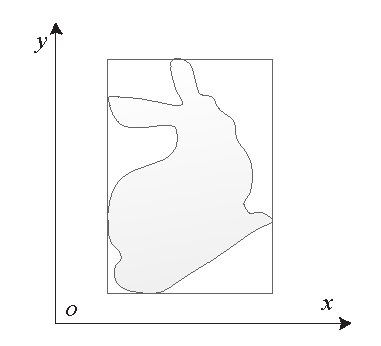
\includegraphics[width=0.2\textwidth]{figures/bunny-2d-AABB.eps}
        }
        \subfloat[\scriptsize OBB]
        {
            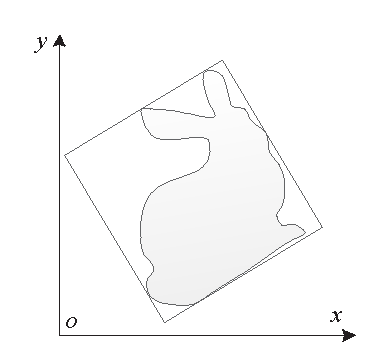
\includegraphics[width=0.2\textwidth]{figures/bunny-2d-OBB.eps}
        }
       \subfloat[\scriptsize Sphere]
        {
           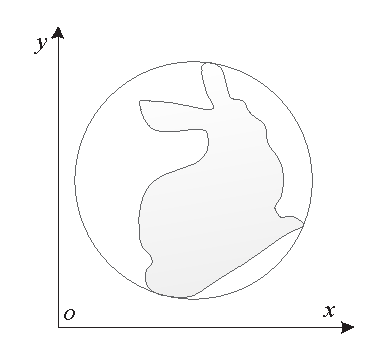
\includegraphics[width=0.2\textwidth]{figures/bunny-2d-Sphere.eps}
        }%\linebreak
        \subfloat[\scriptsize $k$-DOP]
        {
           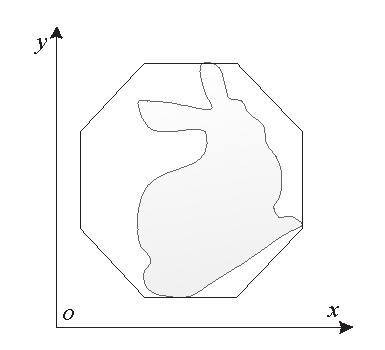
\includegraphics[width=0.2\textwidth]{figures/bunny-2d-8DOP.eps}
        }
        \subfloat[\scriptsize 凸包]
        {
           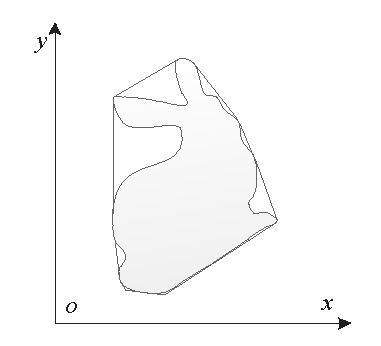
\includegraphics[width=0.2\textwidth]{figures/bunny-2d-Convexhull.eps}
        }
        \end{minipage}
        \caption{不同种类的包围体}
        \label{chart:exps:tightness}
        \end{figure}
        \vspace{-1em}
      其他:Tribox、Swept-sphere、 Sphere-shell、Zonotopes、圆柱形、圆锥、椭球形等等。
      
      \note{
        上面这几个就是最常见的凸包围体。最常见的沿坐标轴方向的AABB包围盒,带方向的包围盒OBB,包围球,k面的凸包围体(k-DOP),和凸包,还有一些比较特定领域用的圆柱、圆锥形、椭球形等等。
        其中k-DOP是综合来看不错的包围体,因为可以通过k来调节包围体的简单性和紧致性来满足不同应用的需求。
      }
  }

      \frame{
   \frametitle{本文目标}
     \footnotesize
     综合来看,\textbf{$k$-DOP}\footfullcite{klosowski1998efficient}的方向\textbf{固定}且为\textbf{有限的偶数},不同模型其截面方向一致, \textbf{不够紧致};\\ 
     而凸包很(最)紧致,但面片数量太多,构造复杂度$O(n\log n)$。
    \begin{block}{本文凸包围体的目标}
      \hspace{-1em}   \begin{minipage}{\textwidth}
    \begin{description}
      \item[紧致:] 能够自适应模型,根据模型形状特点有不同的方向;
      \item[快速:] 生成凸包围体的速度要快,利用~GPU~加速;
      \item[灵活:] 通过参数~$k$~调节凸包围体的简单性和紧致程度。
    \end{description}
  \end{minipage}
    \end{block}

       \note{
本文提出的 k-CBP 与 k-DOP 不同之处在于:
(1) k-DOP 中 k 值通常仅局限于少数几个,例如 k = 6,8,14,18,20,26 等\cite{klosowski1998efficient}文
献\cite{abenchmarking2007}最大支持 k = 46),且 k-DOP 中方向是成对平行的,k 值是偶数,而 k-CBP 中
的 k 理论上可以是任意的,奇偶都可以;
(2) k-DOP 中的凸多面体方向是固定的即 k 值确定之后,不管输入模型的点集
分布如何, k-DOP 的方向始终保持一致,本文则提出了一种能够自适应模型的算
法使得构造的凸包围多面体足够紧致;
(3) k-CBP 中 k 取值灵活,必须找出一种算法生成 k 个法向,比只有少数几个可直接通过枚举方向的 k-DOP 取值更复杂。
通过更加紧致的 k-CBP 去近似原始模型,能够达到更好的精度,且输入 k 值
可以自由控制,为其能够用于碰撞检测等应用提供足够大的灵活性。
       }
  }

  \subsection{碰撞检测算法}
   \frame{
   \frametitle{\subsecname~ }
    
   \begin{block}{碰撞检测算法}
     许多应用的基础,例如在~3D~游戏,物理仿真,机器人,虚拟现实等领域中\footfullcite{ericson2005real}。
   \end{block}

   \begin{block}{分类}
     \begin{description}
       \item[加速结构:] SPT(如四叉树、KD~树等)~v.s~\textbf{BVH}(OBB树、$k$-DOP树等)
       \item[表现形式:] \textbf{刚体}~v.s~可变形,凸体~v.s~凹体,CSG~v.s~参数曲面~v.s~\textbf{多边形网格}
       \item[碰撞环境:] \textbf{成对}~v.s~\textbf{多体},\textbf{静止}~v.s~\textbf{运动},\textbf{离散}~v.s~连续
     \end{description}
   \end{block}
   
   \note{
    (介绍PPT后),本文后面的实验就是基于BVH的,不可变形的三角网格。//现在研究较多的是连续的可变形的碰撞检测布料模拟头发模拟等。
   }
  }

  \frame{
    \frametitle{基于~BVH~的碰撞检测算法}
    \begin{columns}[onlytextwidth]
      \begin{column}{0.35\textwidth}
        \vspace{-1.5em}
        \begin{figure}[htbp]
            \begin{center}
            \begin{boxedminipage}{1\textwidth}
            \subfloat{\label{lbl:bvh-bunny-center-0.png}}
              {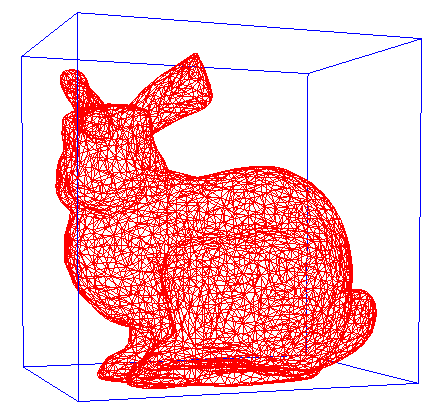
\includegraphics[height=1.4cm]{bvh-bunny-center-0.png}}
            \subfloat{\label{lbl:bvh-bunny-center-1.png}}
              {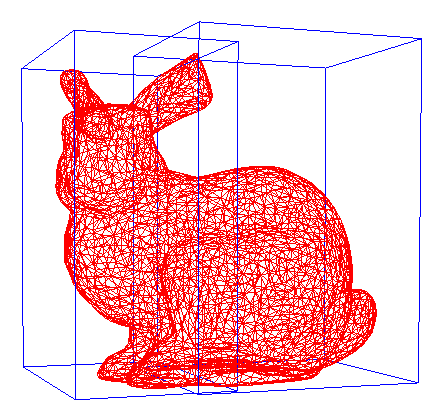
\includegraphics[height=1.4cm]{bvh-bunny-center-1.png}}
            \\
            \subfloat{\label{lbl:bvh-bunny-center-2.png}}
              {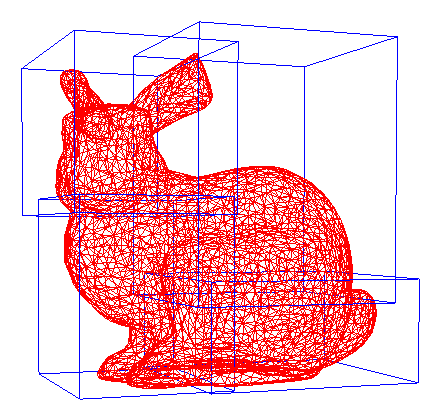
\includegraphics[height=1.4cm]{bvh-bunny-center-2.png}}
            \subfloat{\label{lbl:bvh-bunny-center-3.png}}
              {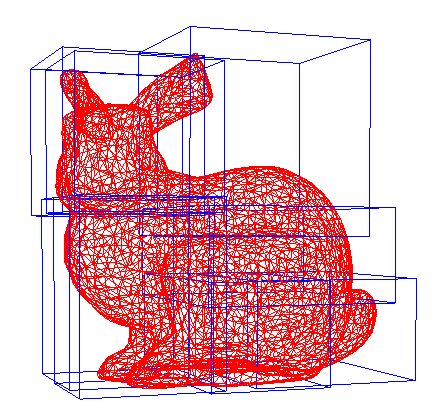
\includegraphics[height=1.4cm]{bvh-bunny-center-3.png}}
            \\\hspace{0.5cm}
            \subfloat{\label{lbl:bvh-bunny-center-4.png}}
              {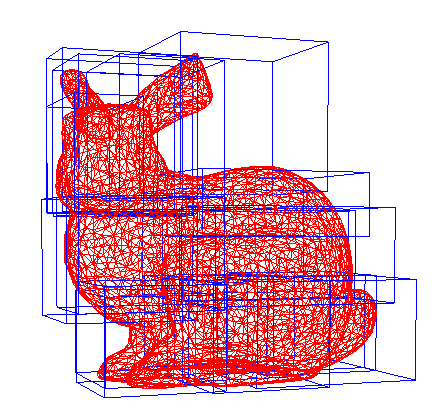
\includegraphics[height=1.5cm]{bvh-bunny-center-4.png}}
            \subfloat{\label{lbl:bvh-bunny-center-5.png}}
              {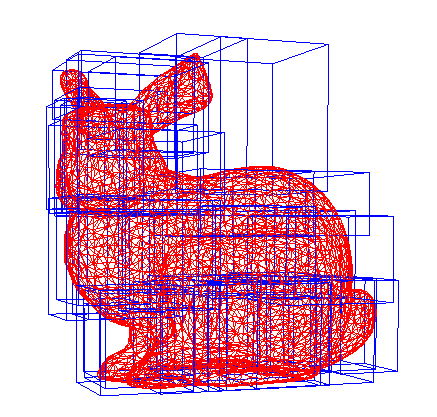
\includegraphics[height=1.5cm]{bvh-bunny-center-5.png}}
            \\
            \subfloat{\label{lbl:bvh-bunny-center-6.png}}
              {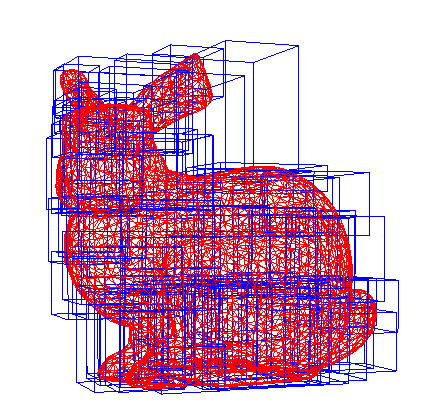
\includegraphics[height=1.5cm]{bvh-bunny-center-6.png}}
            \subfloat{\label{lbl:bvh-bunny-center-7.png}}
              {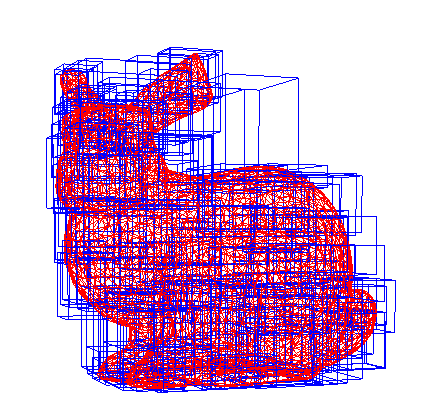
\includegraphics[height=1.5cm]{bvh-bunny-center-7.png}}
            \end{boxedminipage}
            \vspace{-0.5em}
          \caption{八层~BVH~示例}
          \label{lbl:bvh-example}
          \end{center}
          \end{figure}
      \end{column}
      \hspace{0.5em}
      \begin{column}{1.2\textwidth}
      \vspace{0.2em}
         \scalebox{0.5}{
              \begin{minipage}{1.0\textwidth}
      \vspace{-2em}
           \begin{algorithm}[H]
              \caption{自顶向下层次遍历~BVH~}
              \label{alg:traverse-bvh-tree}
              \begin{algorithmic}[1]
              \Require
              两个~BVH~树的根节点~$node_1$,$node_2$
              \Ensure
              模型是否相交
              \Function {TraverseBVHTree}{$node_1, node_2$}
                \If{$node_1.bv \cap node_2.bv = \emptyset$}
                  \State \Return{\textbf{False}}
                  \Comment{包围体重合测试, 包围体不相交直接返回}
                \Else
                    \If {$node_1.children = \emptyset$}
                         \If {$node_2.children = \emptyset$}
                         \State \Comment{最底层叶子节点原生几何相交测试}
                         \State \Return {\Call{CheckIntersection}{$node_1.primitives, node_2.primitives$}}
                         \Else
                            \ForAll {$child \in node_2.children$}
                            \State \Call{TraverseBVHTree}{$node_1, child$} \Comment{递归调用}
                            \EndFor
                         \EndIf
                    \Else
                         \ForAll {$child \in node_1.children$}
                         \State \Call{TraverseBVHTree}{$child, node_2$}  \Comment{递归调用}
                         \EndFor
                    \EndIf
                \EndIf
              \EndFunction
              \end{algorithmic}
              \end{algorithm}
              \end{minipage}
            }
      \\
      \scriptsize \hspace{1em}代价函数: $T_{cost} = n_v * C_v + n_p * C_p + (n_u * C_u)$(运动)
      \end{column}
    \end{columns}
    \note{
      基于包围体树的碰撞检测算法, 一般首先都会初始化环境然后构建层次结构的包围体树,碰撞检测时从顶层开始逐渐往下层遍历,到最底层叶子节点后开始三角网格模型相交测试,
      当发现三角网格相交后立即终止遍历,确定模型发生碰撞。
      评价碰撞检测算法的指标一般用上面这个公式来衡量,其中nv和 np分别表示参与包围体节点相交测试的数量和参与原始几何相交测试的数量,Cv和 Cp则表示相应的平均测试耗费的代价。
      当在运动场景时还需要加上nu和 Cn就是模型旋转或者运动后包围体更新的数量和更新的代价。
      本文算法就是尽早发现包围体不相交的情况,减少np和cp的数量。
    }
}

  % \section{凸包围体生成算法}

    \subsection{问题定义及算法流程}

     \frame{
       \frametitle{问题的定义}
      \begin{columns}[onlytextwidth]
          \begin{column}{0.7\textwidth}
           \begin{block}{凸包围~$k$~面体}%
            $k$-Convex Bounding Polyhedron,简称~$k$-CBP,可通过~$k$~个半空间定义:
              \begin{equation}
              \label{equ:kcbp_definition}
              \left\{
                \begin{array}{l}
                    k\mbox{-CBP} = \mathop  \bigcap \limits_{i = 1}^k \bm{H_i} \\
                    \bm{H_i} = \left\{ {\left. {\bm{p} \in {\mathbb{R}^3}} \right| \bm{n_i} \cdot \bm{p} \le {w_i}} , w_i \in \mathbb{R} \right\},
                \end{array}
              \right.
              \end{equation}
              其中,$\bm{n_i}$~是半空间~$\bm{H_i}$~的法向,方向指向包围体外部,
              $w_i$~是输入点集中沿~$\bm{n_i}$~方向投影的最大值。
           \end{block}
    %        \pgfputat{\pgfxy(5,0)}{\pgfbox[left,top]{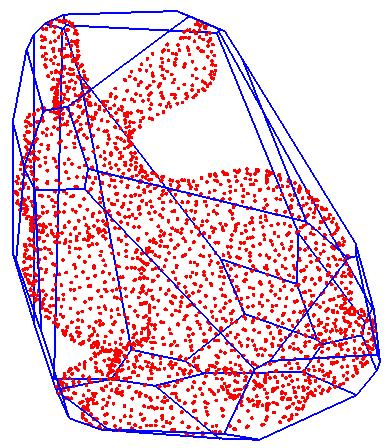
\includegraphics[width=0.25\textwidth]{bunny-34.png}}}
        \end{column}

       %\pgfputat{\pgfxy(7,-1.5)}{\pgfbox[left,top]{
       %  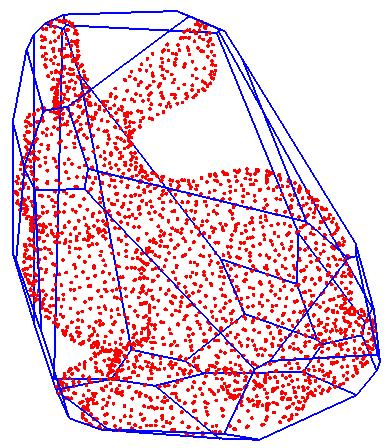
\includegraphics[width=0.25\textwidth]{bunny-34.png}
       %}}
        \begin{column}{0.4\textwidth}
        \begin{figure}
            %\pgfputat{\pgfxy(7,-1.5)}{\pgfbox[left,top]{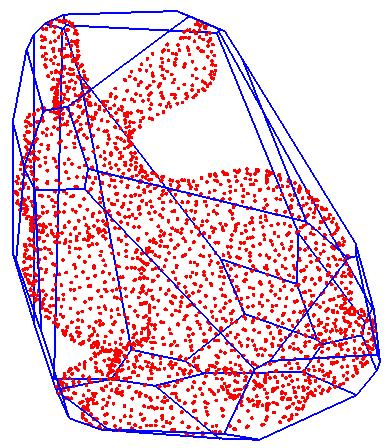
\includegraphics[width=0.8\textwidth]{bunny-34.png}}} %%cannot use caption for pgfputat
            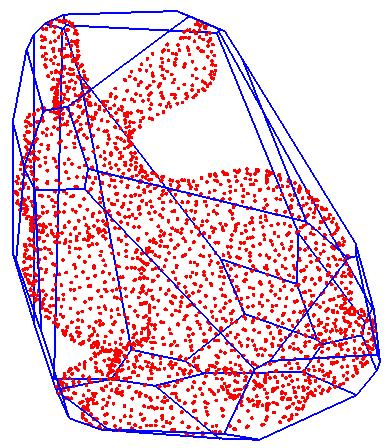
\includegraphics[width=0.8\textwidth]{bunny-34.png}
            \caption{34-CBP}
        \end{figure}
        \end{column}
      \end{columns}

      \note{这是凸包围多面体的定义,其实就是空间中将模型包裹起来的k个平面,右图就是一个k=34的例子。
      其实这个问题的关键就是如何确定这些平面的方向。
      }
    }

       \frame{
       \frametitle{算法流程}
       \begin{block}{构造$k$-CBP~算法流程图}
        \begin{figure}
        \centering
        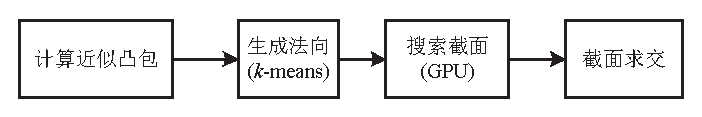
\includegraphics[width=4.0in]{kcbp-flowchart-x-aix.eps}
        \label{lbl:kcbp-algorithm-flowchart}
        \end{figure}
    \end{block}
    \begin{block}{关键步骤}
          \begin{description}
             \item[定法向:]结合近似内凸包和~$k$-means;
             \item[搜截面:]GPU~中沿各法向搜索切点构造截面;
             \item[求交点:]截面对偶映射求得交点。
          \end{description}
    \end{block}

    \note{这是本文构造凸包围多面体的算法流程图,关键就是这3步。\\
      定法向:方向的好坏直接决定最后多面体的紧致程度,本文结合了近似内凸包和kmeans聚类算法来确定法向。\\
      搜截面:因为法向确定后,搜索截面的过程各个法向之间相互独立互不影响,因此可以较方便用GPU加速。\\
      求交点:确定好平面后直接求交即可得到k-cbp的顶点。
    }
}

  \subsection{截面法向的生成}

    \frame{
        \frametitle{近似凸包的构造}
        \begin{figure}
        \vspace{-3mm}
        \subfloat[分组]
        {
           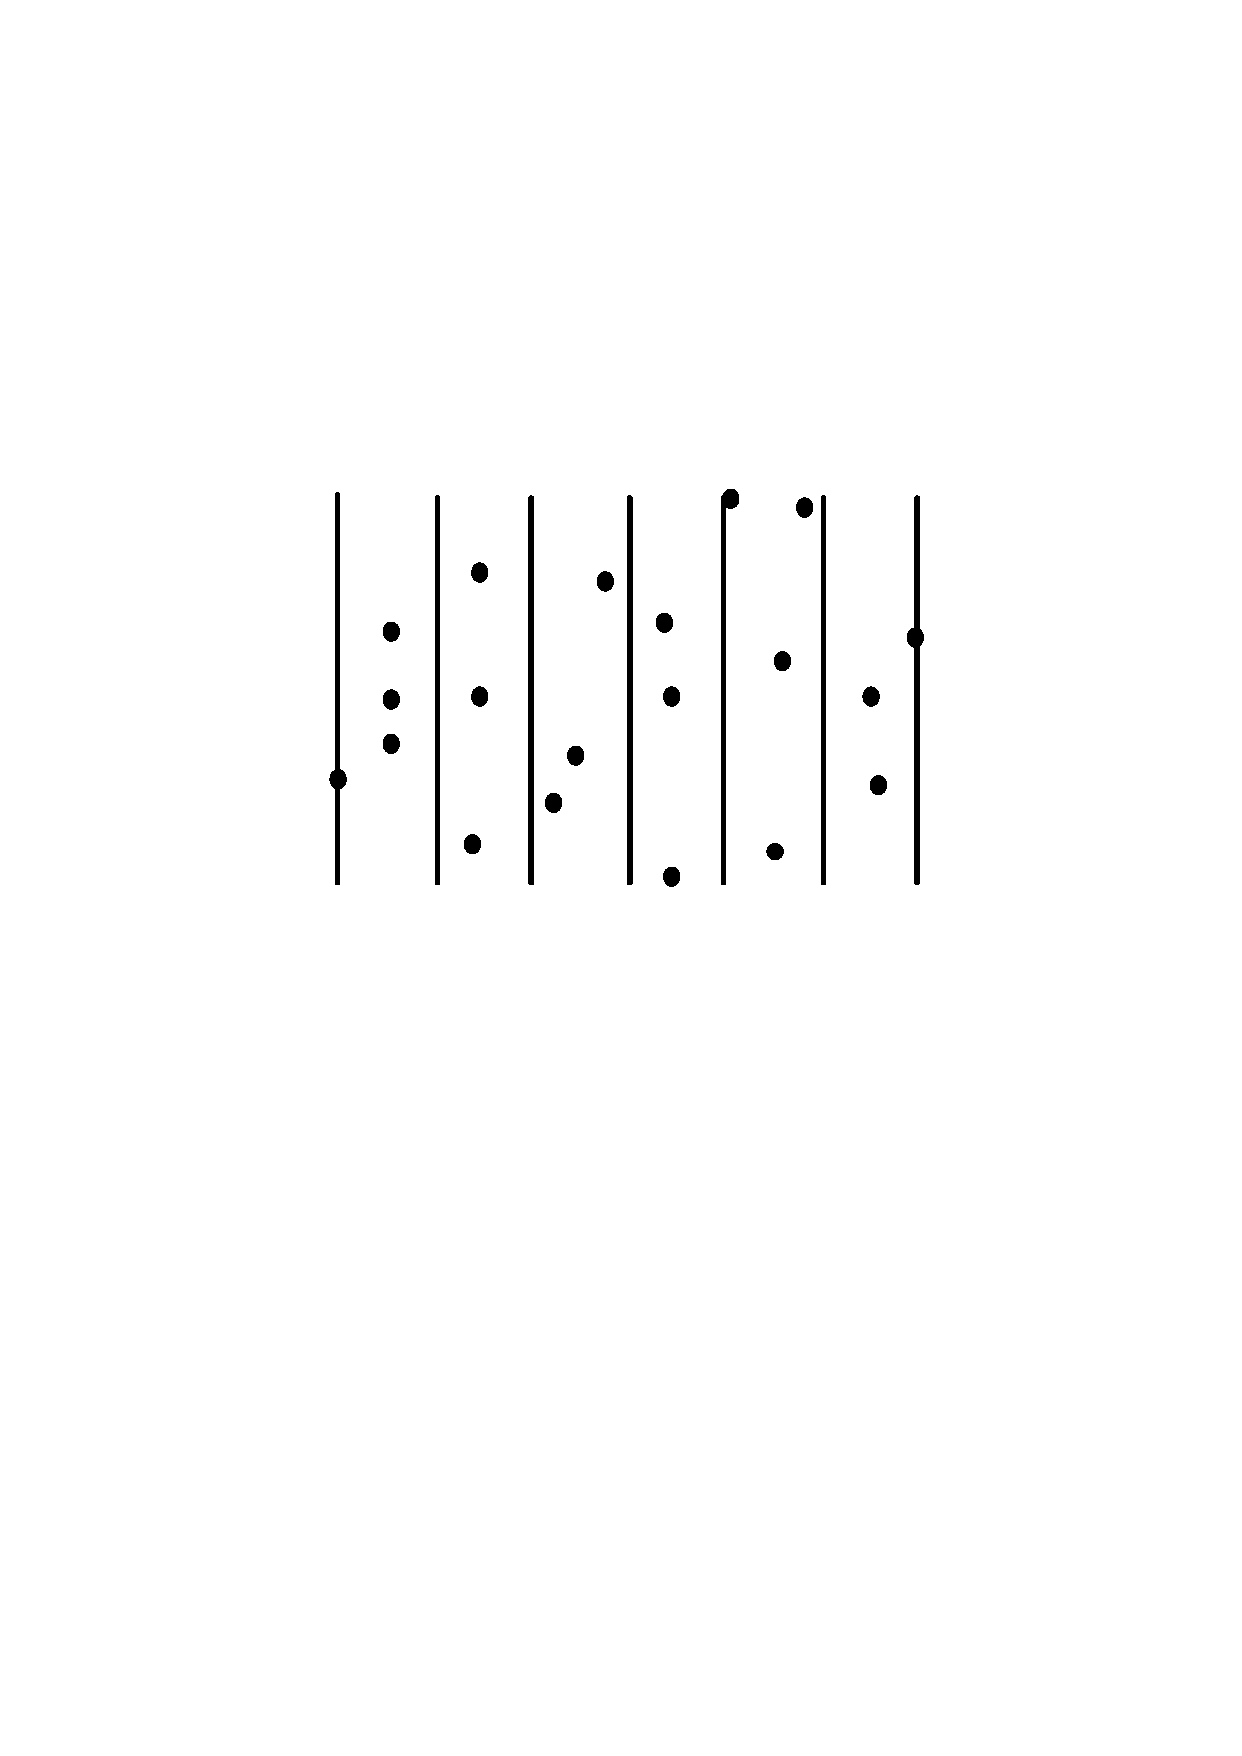
\includegraphics[width=0.28\textwidth]{figures/approximate-convexhull-step1.pdf}
        }\hspace{2mm}
        \subfloat[选极值点]
        {
            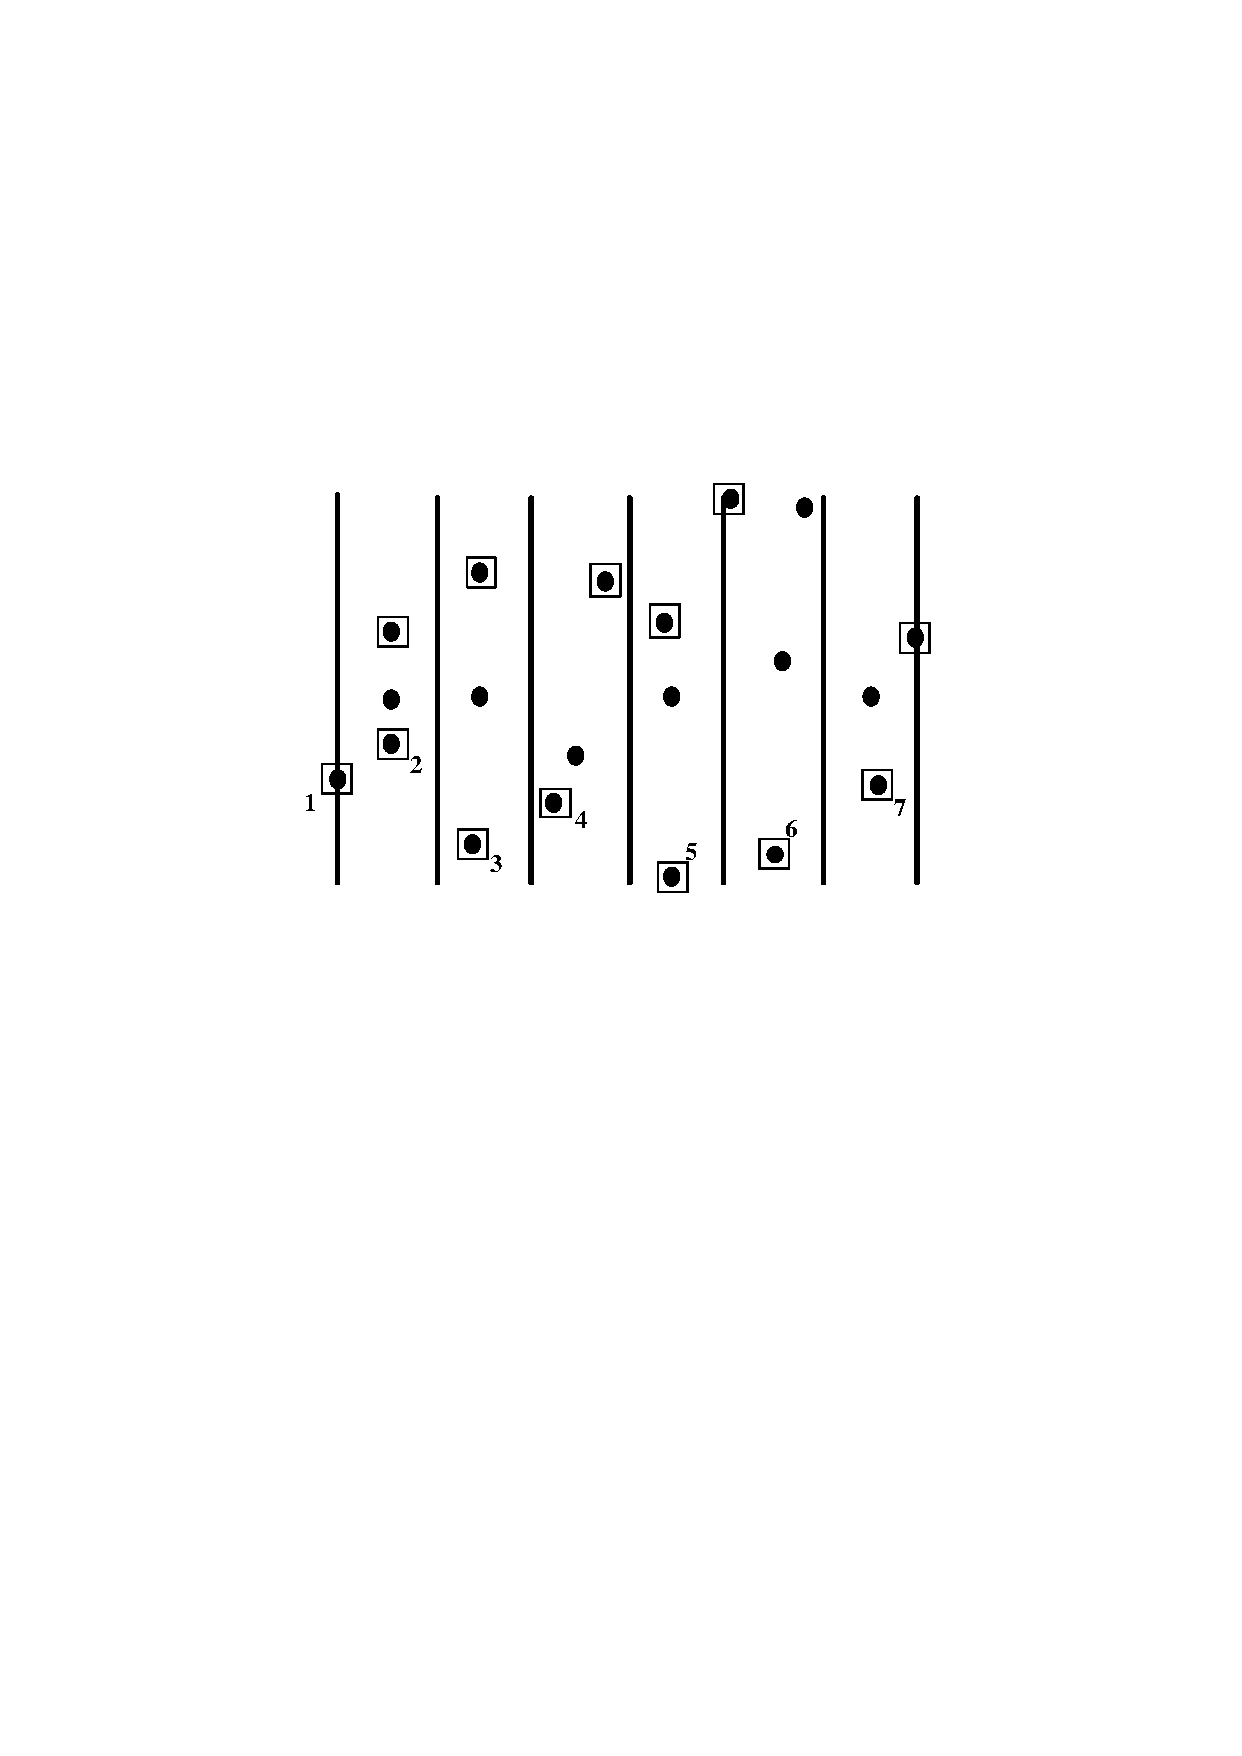
\includegraphics[width=0.28\textwidth]{figures/approximate-convexhull-step2.pdf}
        }\hspace{2mm}
        \subfloat[连线]
        {
           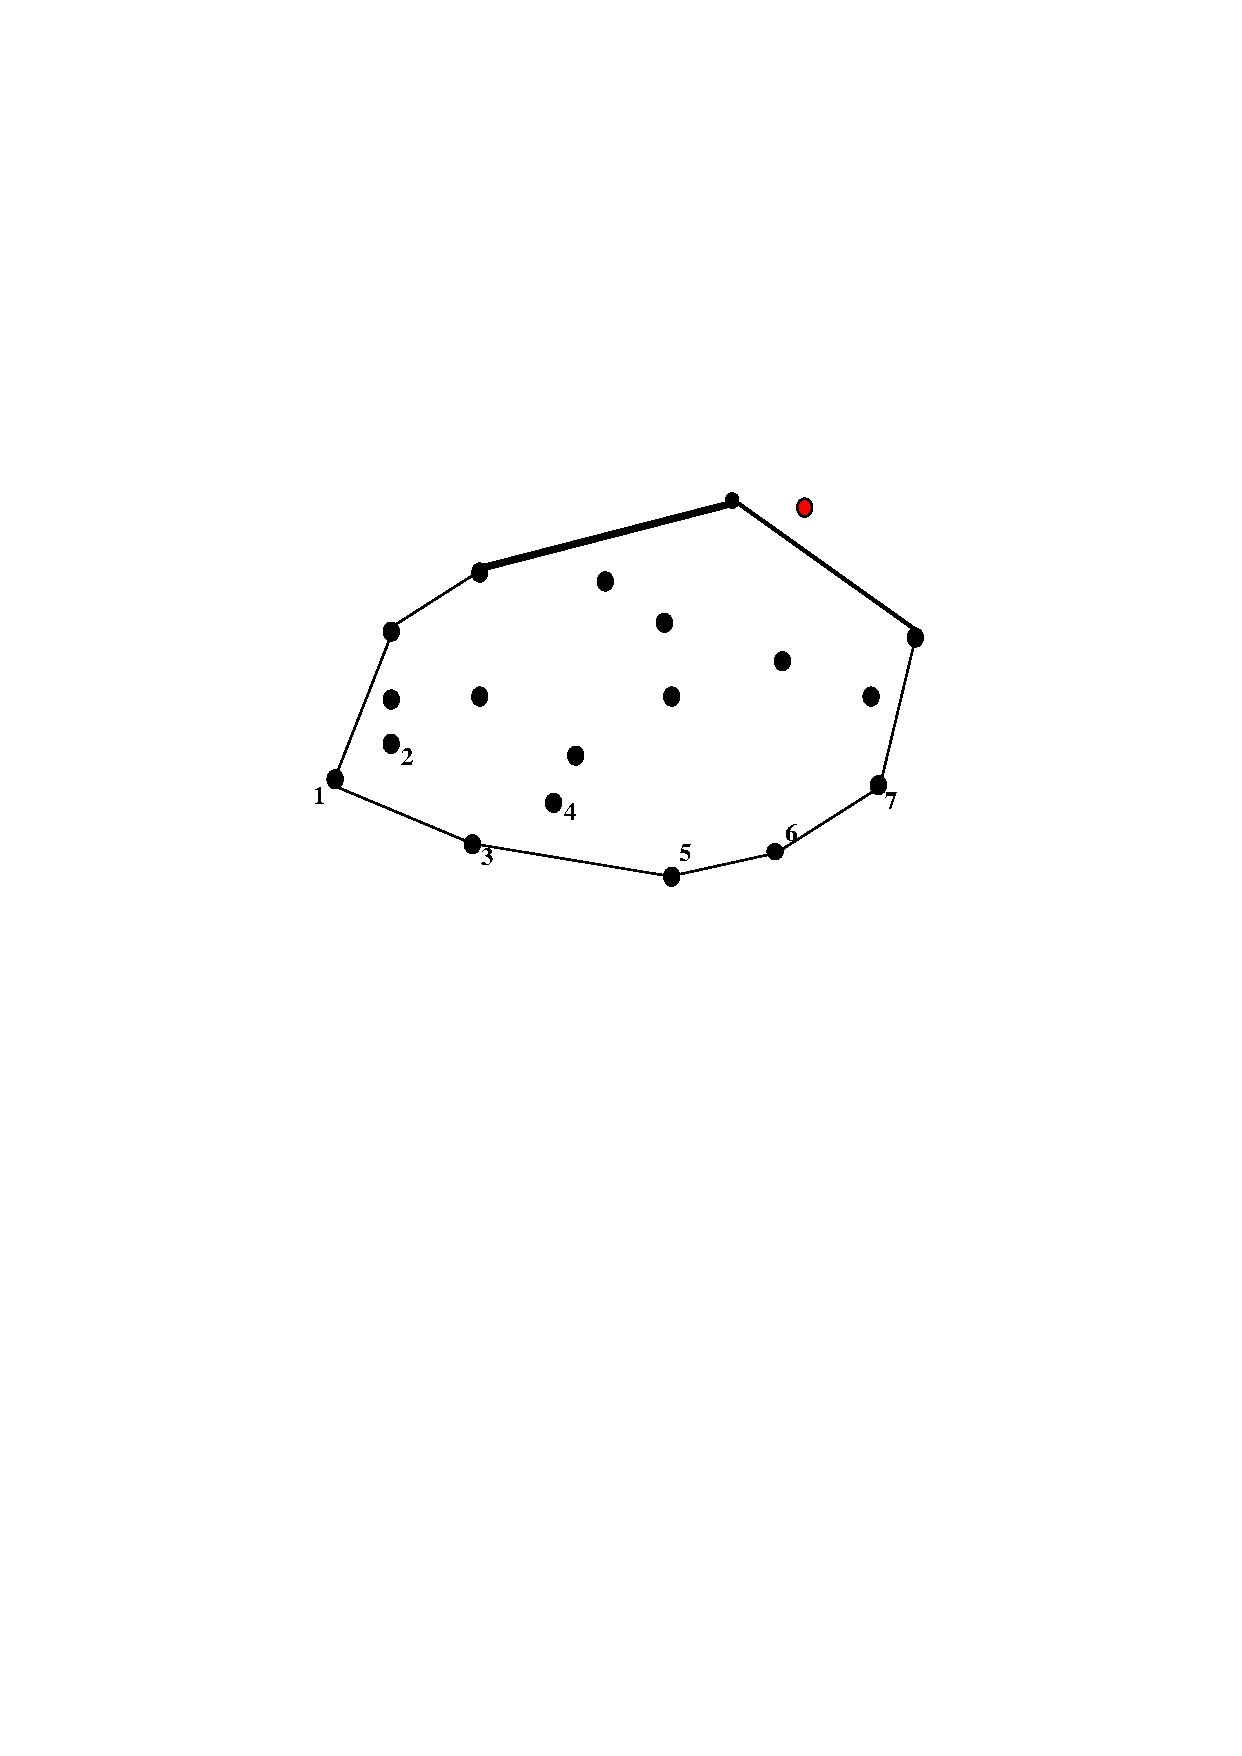
\includegraphics[width=0.28\textwidth]{figures/approximate-convexhull-step3.pdf}
        }
        \caption{二维近似内凸包的构造}
        \label{lbl:ach-2d}
        \end{figure}
        \vspace{-4mm}
        构造近似内凸包\footfullcite{bentley1982approximation},算法复杂度为~$O(n+\lambda)$,扩展到三维为~$O(n+\lambda^2 \log \lambda)$,然后利用$k$-means 聚类。
        
        \note{
          以二维为例,近似内凸包构造分为3个步骤,先分组,然后选出每组的极值点,最后将极值点按条件连接起来即可。此算法时间复杂度为~$O(n+\lambda)$,$\lambda$为分的组数。\\
          三维情况类似。\\
          得到近似凸包后,根据凸包面片的方向作为参与kmeans聚类算法的点集。
        }
    }
    \frame{
        \frametitle{$k$-means 聚类}
      \begin{figure}
        \vspace{-2mm}
        \subfloat[]
        {
           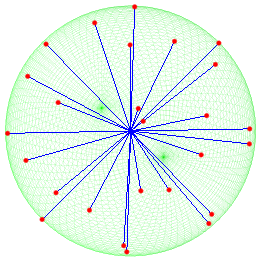
\includegraphics[width=0.25\textwidth]{kmeans-init-normals-26.png}
        }
        \subfloat[]
        {
            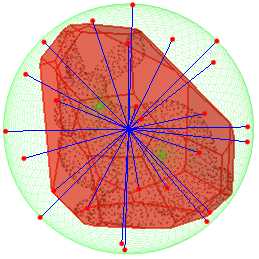
\includegraphics[width=0.25\textwidth]{kmeans-init-normals-26-for-bunny.png}
        }
        \subfloat[]
        {
           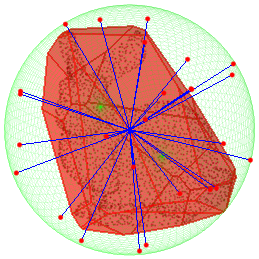
\includegraphics[width=0.25\textwidth]{kmeans-cluster-normals-26-for-bunny.png}
        }
        \vspace{-2mm}
        \caption{通过聚类确定法向}
        \label{lbl:gen-fixed-normals}
        \end{figure}
        \begin{description}
         \item[初始方向:]均匀分布;
         \item[距离度量:]余弦;
         \item[中心更新:]
   中心点:$\bm{c_i}=\frac{\sum_{i=1}^{i=n} \omega_i \cdot \bm{n_i} } {\sum_{i=1}^{i=n} \omega_i}$,权重$\omega_i$为面片面积。
        \end{description}

        \note{
          聚类算法需要关注下面3个问题,一是初始的方向,本文的算法采用均匀分布的方式确定,如图a,在球面上均匀分布k个点,球心和点的连线作为初始方向,图中k=26。 \\
          然后是类与类之间的距离如何度量,用余弦的方式可以使方向相近的点聚到一类。\\
          中心点的更新,以面片所在方向的面积作为权重,使得最后结果靠近面片较大的方向。图c为聚类后的结果,比图b紧致15\%左右。
        }
    }

  \subsection{搜索截面及求交}
    \frame{
    \frametitle{搜索截面}
    \begin{block}{截面=法向+点}
     法向已得,求投影点:对每个法向~$\bm{n_i}$,从输入模型的所有点中寻找最大投影值的点作为切点。
	时间复杂度为~$O(k\cdot n)$, 其中~$k$~为法向数量,$n$~为模型所含点数。
   \end{block}
   \begin{block}{并行可行性}
	各法向的计算相互独立, 借助~GPU~并行加速。
	典型GPU并行平台:着色器(GLSL为例)和基于 GPU 的通用计算框架(CUDA为例)。
	\end{block}

    \note{
     方向确定后,直接沿着方向搜索切点即可。因为各方向搜索过程相互独立,所以可借助GPU加速,本文采用两种典型的GPU加速平台,一种是OpenGL着色语言为代表的着色器平台,另一种是GPGPU通用计算框架CUDA。
    }
    }
    
    \frame{
    \frametitle{GLSL实现}
	     \begin{columns}[onlytextwidth]
     		 \begin{column}{0.5\textwidth}
		 \begin{figure}
	    		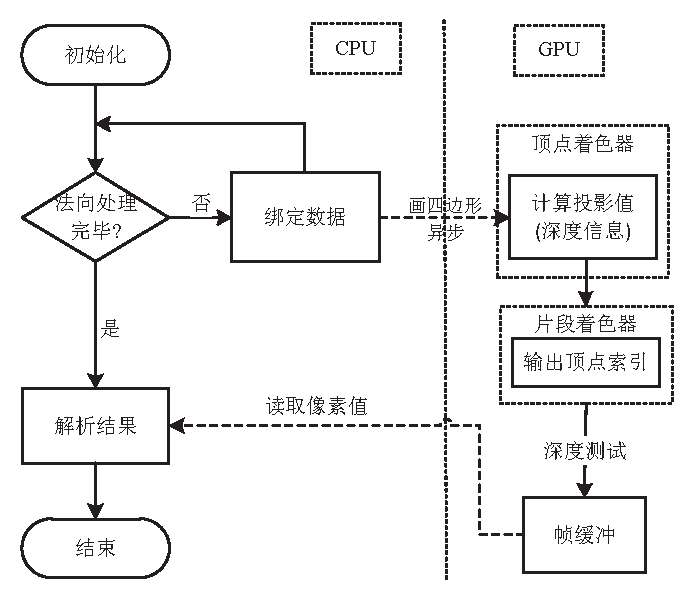
\includegraphics[width=\textwidth]{shader-z_buffer.eps}
	    		\caption{基于Z Buffer算法流程图}
		\end{figure}
	    	\end{column}
          \hspace{1em}
           \begin{column}{0.5\textwidth}
		   	\begin{figure}
		 	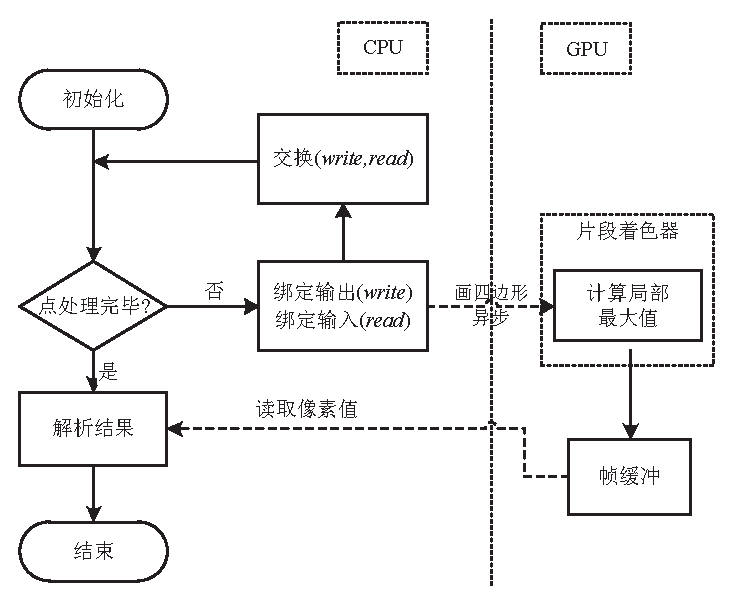
\includegraphics[width=\textwidth]{shader-rtt_pp.eps}
	    		\caption{基于乒乓技术算法流程图}
			\end{figure}	
	    	\end{column}
       	\end{columns}

        \note{
          \scriptsize
          GLSL中,本文提出了两种算法,
          一种是利用OpenGL的深度测试,深度测试的目的是决定哪个片段将要保留下来,默认情况下,最前面即有较小(或较大,可设置)的 z 坐标值的片段将通过测试被保留下来。每个片段的深度信息保存在深度缓冲中,当新的片段通过测试后将更新缓冲中的值。在顶点着色器中,将所有点的 x,y 坐标值设为一样,并将该点在法向上的投影作为 z 值即深度值,所有点经过深度测试后将只有 z 值最大的点被保留下来,该点就是沿着这个法向的切点。这样经过k次渲染即可找到所有的k个切点。\\
          \scriptsize
          另外一种是乒乓技术,乒乓技术是需要把前一次运算结果传递给下一次运算用来作为后继运算的输。算法将输入点分成 x 份,每次只处理一份,在当前渲染过程中,找出在该批点集中沿着所有法向投影值最大的点,当处理下批点集即下一次渲染时,将与上次局部最大投影值进行比较,若有新的投影最大值就更新,如此反复 x 次,当所有点都被处理完毕后得到沿着所有法向投影最大值的点即切点。所以这个算法对k不是很敏感,因为k相对较小时,GPU一次总能处理k个方向,这点从后面的实验结果也能看出。
        }
   }
    
    \begin{frame}
    \frametitle{CUDA实现}
    \vspace{-1em}
	    \begin{figure}
	    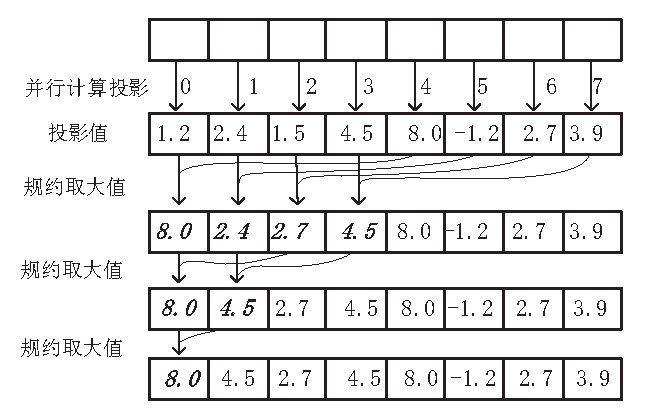
\includegraphics[width=2.5in]{gpureduction.eps}
	    \caption{并行规约求最大投影值}
	    \label{lbl:reduction-getmax}
	    \end{figure}
	    \vspace{-1.5em}
	    \small 
	    将输入点交给数量为~$t$~的线程计算点积得到投影值,
 线程~$i$~和~$i+t/2$~比较选取较大者,经~$\log_2t$~次比较可得最大值。OpenCL等并行计算框架类似。
  
 \note{
      CUDA实现中原理如上图所示,将输入点交给数量为~$t$~的线程计算点积得到投影值,线程~$i$~和~$i+t/2$~比较选取较大者,经~$\log_2t$~次比较可得最大值。
      这种规约方式在其他GPGPU框架中也类似,如OpenCL等。
 }
    \end{frame}

        \frame{
    \frametitle{求交算法}
      \begin{block}{直接枚举}
      通过枚举所有每~3~个平面交于~1~点的情况,然后排除在平面外部的交点,剩下的构成~$k$-CBP~的顶点,时间复杂度为$O(k^3)$。
      \end{block}
      \begin{block}{对偶映射}
        法向~$\bm{n}(a,b,c)$~ + 平面上点~$\bm{p}(x_0,y_0,z_0)$ $\Rightarrow$ 平面方程~$ax + by + cz = ax_0 + by_0 + cz_0=d$, $d \neq 0$ \\
        对偶点为~$\bm{p'}(a/d, b/d, c/d)$,对~$k$~个映射点求凸包,凸包平面映射回原来的交点,时间复杂度为$O(k\log k)$\footfullcite{dengcg}。
      \end{block}
      
      \note{
        确定平面后,接下来就是求每个平面上的交点。一种比较直接的算法是通过枚举所有每~3~个平面交于~1~点的情况,然后排除在平面外部的交点,剩下的构成~$k$-CBP~的顶点,时间复杂度为$O(k^3)$。
        通过计算几何中的对偶映射技术可以将复杂度降低到$O(k\log k)$。
      }
    }

  \subsection{实验结果与分析}

  %\subsubsection{凸包围多面体的生成速度}

    \frame{
      \frametitle{生成$k$-CBP的效率:GLSL实验结果}
      \vspace{-1em}
      \begin{figure}[htbp] % use [htbp] to fix the position
      \vspace{-8mm}
      \subfloat %Apple模型(8118个点)
      {  
         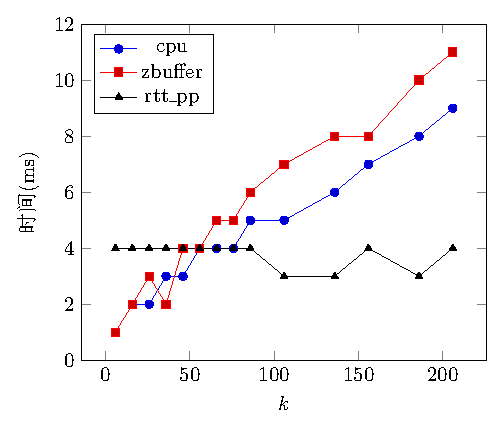
\includegraphics[width=\fourgraphicswidth\textwidth,page=1]{shadertime.pdf}
      }
      \subfloat % Buddha模型(31232个点)
      {  
          \includegraphics[width=\fourgraphicswidth\textwidth, page=2]{shadertime.pdf}
      }\vspace{-8mm}\linebreak %强制换行
        \vspace{-3mm}%
      \subfloat % Alice模型(224291个点)
      {  
         \includegraphics[width=\fourgraphicswidth\textwidth, page=3]{shadertime.pdf}
      }
      \subfloat % Bugatti模型(1010815个点)
      {  
         \includegraphics[width=\fourgraphicswidth\textwidth, page=4]{shadertime.pdf}
      }
      \caption{\tiny Apple(8k), Buddha(31k), Alice(224k), Bugatti(1011k)}
      \label{fig:chart:exps:shadertime}
      \end{figure}

      \note{
        这是基于OpenGL着色语言实现的实验结果。
      从实验结果可以看出,当模型规模不大时,如左上图所示的含有8千多个点的~Apple~模型,
Z Buffer~算法和传统的~CPU~算法差别不是很大,因此在实际应用中当模型规模较小时可直接用~CPU~计算即可。
随着输入模型所含有点的数量规模的增加,CPU~和~GPU~运行时间之间的差距也越来越大。
当多面体面数增加即~$k$~的增大时,在~Z Buffer~算法中,需要更多的绘制次数,因此其运行时间也有所增加,而在基于乒乓技术的算法中,当点规模一定时,$k$~的变化对最后运行时间影响不明显,因此当较大的~$k$~时,这种算法更快。
      }
    }

    \frame{
      \frametitle{生成$k$-CBP的效率:CUDA实验结果}
      \vspace{-1em}
        \begin{figure}
        \vspace{-8mm}
        \subfloat%[\tiny Budda(31232 points)]
        { 
           \includegraphics[width=0.35\textwidth,page=2]{figures/cudatime.pdf}
        }
        \subfloat%[\tiny Dinosaur(40277 points)]
        { 
            \includegraphics[width=0.35\textwidth, page=3]{figures/cudatime.pdf}
        }\vspace{-8mm}\linebreak %强制换行
        \vspace{-3mm}%
       \subfloat%[Alice(224291 points)]
        {
           \includegraphics[width=0.35\textwidth, page=4]{figures/cudatime.pdf}
        }
        \subfloat%[Bugatti(1010815 points)]
        {
           \includegraphics[width=0.35\textwidth, page=5]{figures/cudatime.pdf}
        }
        \caption{\tiny Budda(31k),Dinosaur(40k),Alice(224k), Bugatti(1011k)}
        \label{chart:exps:cputime}
        \end{figure}

        \note{
         这是CUDA的实验结果,
        图中横纵坐标分别代表多面体面数和运行时间, 其中虚线代表搜索截面的过程, 实线为构造凸包围多面体总体耗时. 当模型点数量较大时, 搜索截面的过程占据了算法绝大多数时间, 且随着凸包围多面体的面数~$k$~ 值增加而线性增长, 这与搜索截面时间复杂度($O(k\cdot n)$)一致, 截面求交过程的时间复杂度为$O(k\log k)$,
当点数量极大时, 实线虚线几乎重合即求交等步骤耗时相比整体算法而言几乎可忽略.
        }
    }

    \frame{
      \frametitle{生成$k$-CBP的效率:与文献\cite{karlsson2010parallel}算法对比}
        \vspace{-7mm}
        \begin{table} \tiny
        \caption{本文算法与文献\footfullcite{karlsson2010parallel}算法对比}
        \begin{tabular}{p{1.5cm}<{\centering}ccc ccc} %p本身占一列
       \toprule[1pt]
        \multirow{2}{*}{$k$} & \multicolumn{3}{c}{Apple(8118 points)} & \multicolumn{3}{c}{~~~~~Bugatti(1010815 points)}\\
        %\cmidrule(lr){2-4}\cmidrule(lr){5-7}
        %\hline
        %\rowcolor[gray]{0.9} $k$ &
        ~&SSE(ms) & $k$-CBP(ms) &  Speedup &SSE(ms) & $k$-CBP(ms) &  Speedup \\
     \midrule[0.5pt]
        6 & 0.4 & 0.12  & 3.20     & 24.2 & 3.20  & 7.56 \\
        16 & 0.9 & 0.26  & 3.43    & 44.5 & 8.44  & 5.27 \\
        26 & 1.4 & 0.41  & 3.38    & 66.5 & 13.65  & 4.87 \\
        36 & 1.9 & 0.52  & 3.65    & 91.1 & 18.34  & 4.97 \\
        46 & 2.5 & 0.67  & 3.74    & 119.5 & 24.13  & 4.95 \\
        56 & 2.9 & 0.79  & 3.66    & 138.4 & 28.86  & 4.80 \\
        66 & 3.5 & 0.95  & 3.69    & 170.6 & 34.10  & 5.00 \\
        76 & 4.0 & 1.08  & 3.70      & 197.1 & 39.85  & 4.95 \\
        86 & 4.5 & 1.22  & 3.69    & 219.8 & 45.08  & 4.88 \\
        106 & 5.4 & 1.49  & 3.62   & 267.8 & 55.52  & 4.82 \\
        136 &  6.8 & 1.92  & 3.54  & 342.9 & 71.24  & 4.81 \\
        156 &  7.7 & 2.17  & 3.55  & 411.3 & 81.18  & 5.07 \\
        186 &  9.3 & 2.60  & 3.58  & 479.4 & 97.39  & 4.92 \\
        206 &  10.5 & 2.85  & 3.68 & 523.0 & 106.87  & 4.89  \\  
        \bottomrule[1pt]
        \end{tabular}
        \label{tab:exp:sse-time}
        \end{table}
        \vspace{-3mm}
        \scriptsize  当点数量较小时,能够提高~3-4~倍速度,模型变大,加速比更大,Bugatti~模型的提速达到~4$\sim$8~倍。
        
        \note{
          这是和一篇专门讲并行求包围体的算法的论文的对比结果(Swedish瑞典,sigrad会是Eurographics的子会议议题官网说的是the Swedish Chapter of Eurographics),可以看出当点数量较小时,能够提高~3-4~倍速度,模型变大,加速比更大,Bugatti~模型的提速达到~4$\sim$8~倍。
        }
    }

  %\subsubsection{凸包围多面体的紧致程度}
   \frame{
        \frametitle{生成$k$-CBP的紧致程度:$k$-DOP v.s $k$-CBP }
        \begin{figure}
        \vspace{-8mm}
        \subfloat
        {  
           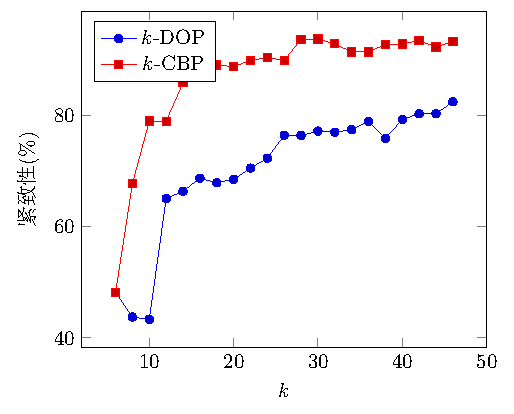
\includegraphics[width=0.35\textwidth,page=1]{figures/tightness.pdf}
        }
        \subfloat
        { 
            \includegraphics[width=0.35\textwidth, page=2]{figures/tightness.pdf}
        }\vspace{-8mm}\linebreak %强制换行
        \vspace{-3mm}%
       \subfloat%[Alice(224291 points)]
        { 
           \includegraphics[width=0.35\textwidth, page=3]{figures/tightness.pdf}
        }
        \subfloat%[Bugatti(1010815 points)]
        {
           \includegraphics[width=0.35\textwidth, page=4]{figures/tightness.pdf}
        }
        \caption{紧致程度对比: \tiny Apple(8k), Budda(31k), Dinosaur(40k), Alice(224k)}
        \label{chart:exps:tightness}
        \end{figure}
        
        \note{
          这是本文算法和k-DOP的对比,较~$k$-DOP~提升 10\% $\sim$ 40\%,下图可视化结果。
        }
    }
    \frame{
      \frametitle{生成$k$-CBP的紧致程度:$k$-DOP v.s $k$-CBP }
      \hspace{3em}
      \vspace{-3em}
      \begin{figure}[H] 
        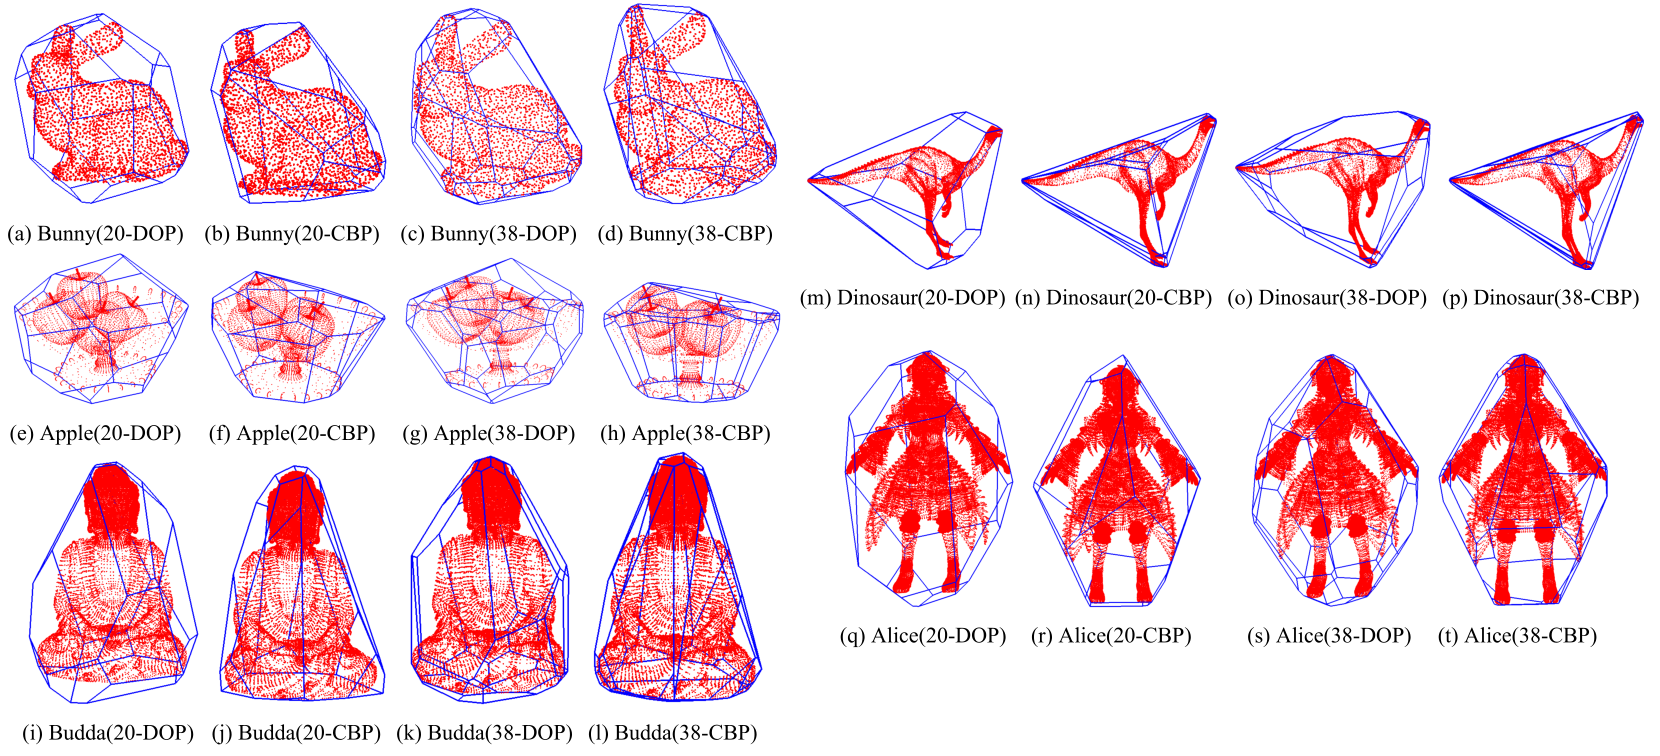
\includegraphics[width=1.05\textwidth]{kCBP-KDOP.png}
      \caption{~$k$-CBP~与~$k$-DOP~对比}
      \label{fig:kdop:kcbp:ui}
      \end{figure}

      \note{
        该图中是不同k值的对比,左边为k-DOP结果,右边为本文结果。从外观上看,确实也紧致了不少。
      }
    }

    \frame{
        \frametitle{生成$k$-CBP的紧致程度:$k$-CBP v.s 凸包 }
        \vspace{-2em}
        \begin{table}
        \scriptsize
        \caption{\label{tab:exp:cgal}$k$-CBP~与~QuickHull~凸包算法比较}
         \begin{tabular}{lcccccl}
          \toprule
          Model & f(CHull)& f($k$-CBP) & $\tau$ ($k$-CBP) & t(CHull(ms)) & t($k$-CBP(ms))\\
          \midrule
          Apple	& 499 & 30 & 93.67\% & 5.5 & 1.30\\ % apple3  自己电脑跑的数据, 之前是用的chengxianyu的电脑.
          Budda	& 1608 & 46 & 92.39\% & 21.3 & 2.86 \\ %  1.0+0.86+1
          Dinosaur	& 1240 & 44 & 93.34\% & 22.6 & 1.99 \\  % 1.0+0.98+0.1
          Alice	& 1332 & 44 & 93.92\% & 85.8 & 8.47\\ % 2+6.48
          Bugatti & 24654 & 44 & 95.06\% & 688.7 & 25.41\\
          \bottomrule
         \end{tabular}
         \vspace{-2mm}
        \end{table}
        \begin{block}{结论}
        \footnotesize 与凸包相比,本文算法在大大简化包围体平面数量的同时能保持较好的紧致程度(Bugatti 凸包面的0.17\%的达到95.06\%紧致程度,构造速度快27倍),下图为可视化结果。
        \end{block}

        \note{
        这是本文算法和CGAL中的凸包的对比,其中f表示面数量,$\tau$的值为紧致程度,紧致程度是用凸包的体积除以凸包围多面体的体积来衡量的。与凸包相比,本文算法在大大简化包围体平面数量的同时能保持较好的紧致程度(Bugatti 凸包面的0.17\%的达到95.06\%紧致程度,构造速度快27倍),下图为可视化结果。
      }
    }

    \frame{
        \frametitle{生成$k$-CBP的紧致程度:$k$-CBP v.s 凸包}
        \begin{figure}
        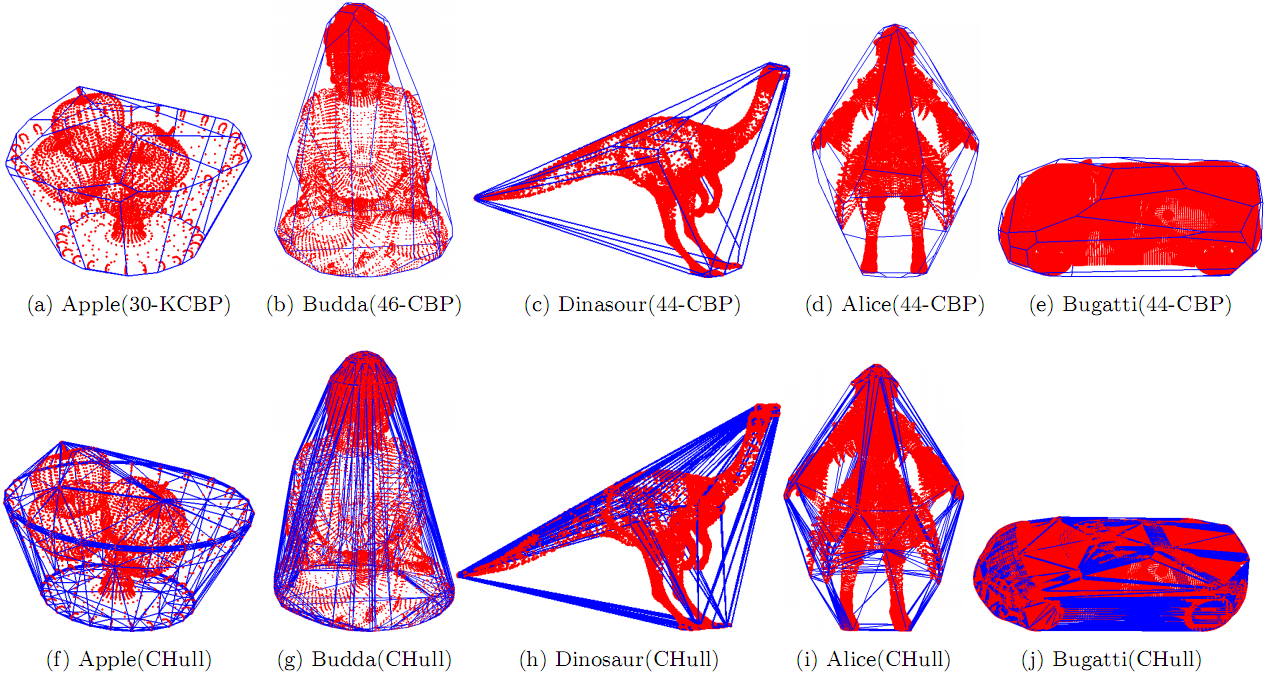
\includegraphics[width=4.0in]{figures/kcbp-convexhull.png}
        \caption{$k$-CBP~与凸包对比}
        \label{pic:exps:ch-kcbp}
        \end{figure}
    }

    \section{基于$k$-CBP~的碰撞检测算法}
    
      \subsection{$k$-CBP~间的相交测试}
      \begin{frame}
        \frametitle{}
        \begin{block}{AABB树法}
          将生成的$k$-CBP视为普通的三角形,实现简单,适用于模型较小的静止碰撞检测场景。
        \end{block}
        \begin{block}{GJK法}
          计算凸多面体之间的最近距离的~GJK~算法\cite{bergen1999fast}。\\
          Minkowski~差,即~$\mathbb{A} - \mathbb{B} = \{ \bm{a} - \bm{b} | \bm{a} \in \mathbb{A}, \bm{b} \in \mathbb{B}\} $。
GJK~算法的核心基础在于若两个凸多边相交,则凸多边形顶点的~Minkowski~差所围成的多边形必包含原点,因为若~$\mathbb{A}$~和
~$\mathbb{B}$~相交即~$\mathbb{A}$~和~$\mathbb{B}$~必含有公共交集,
即至少含有一点同时属于~$\mathbb{A}$~和~$\mathbb{B}$~,该点的~Minkowski~差即为原点~$\bm{O}(0, 0)$。
        \end{block}
      \end{frame}

      \begin{frame}
        \frametitle{二维~GJK~算法示例}
        \begin{figure}[htbp]
        \subfloat[相交]{
          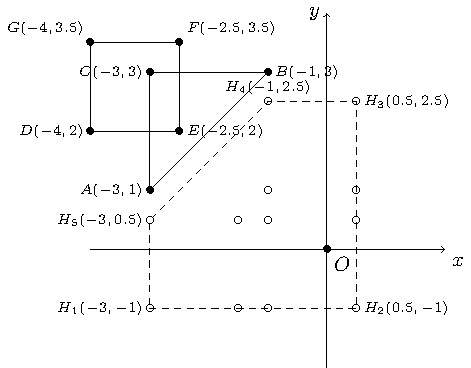
\includegraphics[width=.48\textwidth,page=1]{gjkExample.pdf}
        } 
        \subfloat[不相交]{
          \includegraphics[width=.48\textwidth, page=2]{gjkExample.pdf}
        }
        \end{figure}
      \end{frame}

      \frame{
        \frametitle{GJK~算法}
        \vspace{-2em}
         \begin{columns}[onlytextwidth]
          \begin{column}{0.46\textwidth}
              \begin{figure}[htbp]
          \hspace{-9em}
              \subfloat%[第一步]
              {
                \includegraphics[width=.65\textwidth,page=3]{gjkExample.pdf}
              }\\ \vspace{-3em}\hspace{3em}
              \subfloat%[不相交]
              {
                \includegraphics[width=.65\textwidth, page=4]{gjkExample.pdf}
              }\\ \vspace{-2em} \hspace{-8em}
              \subfloat%[不相交]
              {
                \includegraphics[width=.65\textwidth, page=5]{gjkExample.pdf}
              }
             \end{figure}
          \end{column}
          \begin{column}{1.05\textwidth}
            \vspace{-2em}
            \scalebox{0.5}
            {
              \begin{minipage}{\textwidth}
                \begin{algorithm}[H]
                \caption{基于~GJK~的~$k$-CBP~相交检测算法}
                \label{alg:gjk}
                \begin{algorithmic}[1]
                \Require
                两个~$k$-CBP~$k\texttt{-}CBP_1, k\texttt{-}CBP_2$
                \Ensure
                ~$k$-CBP~是否相交
                \Function{KCBPDetectionBasedOnGJK}{$k\texttt{-}CBP_1, k\texttt{-}CBP_2$}
                    \State $\bm{d} \gets \Call{initNormal}$
                    \State $\bm{D} \gets \Call{Support}{k\texttt{-}CBP_1, k\texttt{-}CBP_2, \bm{d}}$
                    \State $S \gets \{p\}$
                    \State $iter \gets 1 , \bm{d} \gets -\bm{d}$
                    \While{$inter++ < MaxIter$}
                        \State $\bm{D} \gets \Call{Support}{k\texttt{-}CBP_1, k\texttt{-}CBP_2, \bm{d}}$
                        \If {$\bm{D} \cdot \bm{d} < 0 $}
                            \State \Return \textbf{False}
                        \EndIf
                        \State $S \gets S \cup \bm{D}$
                        \State $ contains \gets \Call{CheckContainUpdate}{S, \bm{d}}$ \Comment{检测是否包含原点,对集合~$S$~进行规约,并获取下一次迭代的方向~$\bm{d}$}
                        \If {$contains$}
                            \State \Return \textbf{True} \Comment{包含原点,直接返回相交,否则继续迭代}
                        \EndIf
                    \EndWhile
                    \State \Return \textbf{False} \Comment{达到最大迭代次数,根据需求返回相交或者不相交}
                \EndFunction
                \end{algorithmic}
                \end{algorithm}
              \end{minipage}
          }
          \end{column}
        \end{columns}
      }

      \subsection{三角形间的相交测试}
      \frame{
        %\frametitle{}
            \vspace{-0.5em}
            \begin{figure}[htbp]
              \centering
                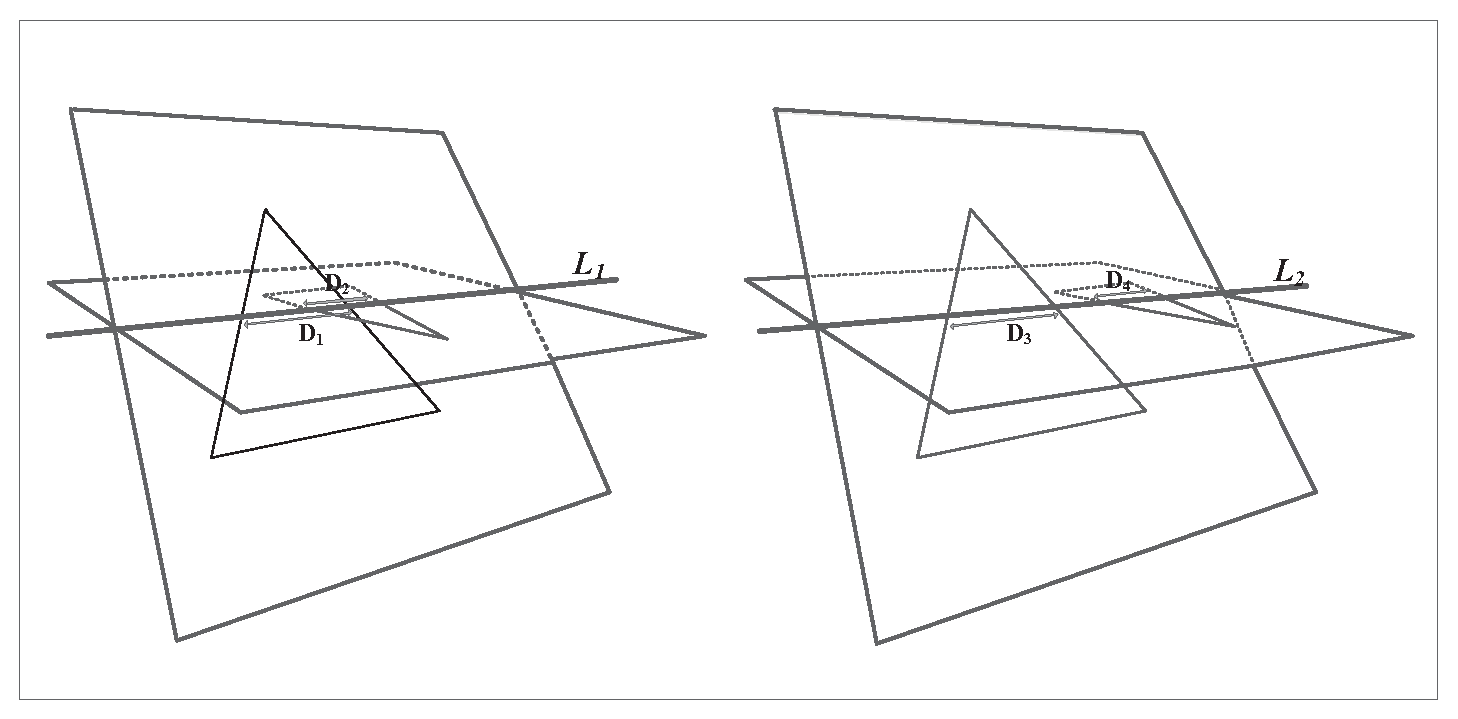
\includegraphics[width=3.0in]{TriangleTriangleTest.eps}
                \caption{两个非共面三角形的位置关系}
              \label{fig:two:triangle:ui}
            \end{figure}
            \vspace{-0.5em}
          \scriptsize 
          三角形~$T_1,T_2$坐标~$\Rightarrow$平面方程$\Pi_1,\Pi_2$$\Rightarrow$~$T_2$~到~$\Pi_1$~的有向距离~$\bm{l}_{1i}, i \in \{1,2,3\}$\cite{Moller1997}:
          \begin{enumerate}[(1)]
            \item 若~$\forall i \in \{1,2,3\}, l_{1i} = 0$,即三角形~$T_2$~的三个顶点到三角形~$T_1$~所在~$\Pi_1$~的距离都为$0$,则两个三角形共面;$\Rightarrow$ 共面三角形求交。
            \item 若~$\forall i \in \{1,2,3\}, l_{1i} > 0$ 或~$\forall i \in \{1,2,3\}, l_{1i} < 0$,即三角形~$T_2$~的三个顶点到三角形~$T_1$~所在~$\Pi_1$~的有向距离同号,则~$T_2$~在~$\Pi_1$~的同一侧,可立即排除相交;
            \item 其他情况,三角形~$T_2$~必交~$\Pi_1$~于一条线段。$\Rightarrow$判断两个区间线段$D_1,D_2$是否相交。
          \end{enumerate}
          
      }

      \subsection{基于$k$-CBP~的碰撞检测算法}

        \frame{
          \frametitle{$k$-CBP的有效性}
            \begin{figure}
            \centering
            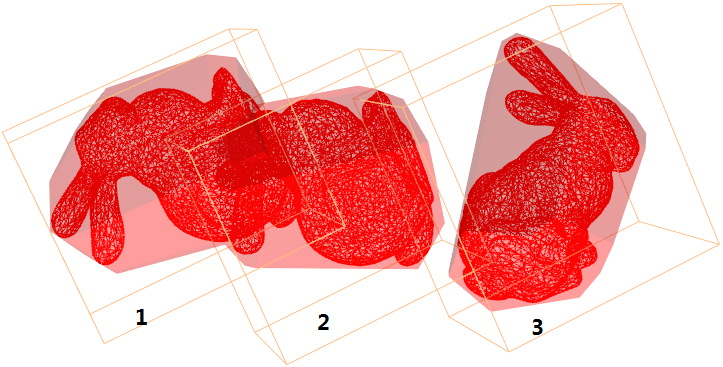
\includegraphics[width=2.5in]{figures/bunny-box-kcbp-collsion-detection-example.png}
            \caption{~$k$-CBP~应用于碰撞检测示例}
            \label{lbl:bunny-box-kcbp-collsion-detection-example}
            \end{figure}

            \footnotesize 图中模型~1~与~2、2~与~3~的包围盒分别相交, 而其~$16$-CBP~仅~1~与~2~相交, 实际模型仅~1~与~2~相交. 
        }
        \frame{
          \frametitle{静止场景碰撞检测算法} 
          \vspace{-2em}
          \begin{figure}[htpb]
            \centering
            \includegraphics[width=0.5\textwidth]{bunny-aabb-bvh-4-layers.pdf}
            \caption{Bunny~模型的~AABB~树形结构(部分)\href{./figures/bv-bunny.gif}{\beamergotobutton{动态图}} } %adobe pdf reader can open it in browser
            \label{fig:bunny:aabb:bvh:toplayer4}
          \end{figure} 
          \vspace{-1em}
           \begin{figure}[htpb]
              \centering
              \includegraphics[width=\textwidth]{collision-detection-flowchart.eps}
              \caption{基于~$k$-CBP~的碰撞检测算法流程图}
              \label{fig:flowchart:cd}
            \end{figure} 
        }
          \frame{
          \frametitle{运动场景碰撞检测算法} 
          \begin{columns}[onlytextwidth]
           \begin{column}{0.35\textwidth}
           \begin{figure}[H]
            \hspace{-4em}
            \includegraphics[width=2.5in]{bunny-2d-AABB-Moving.pdf}
            \caption{\tiny AABB~更新策略图}
            \label{fig:bunny:moving}
          \end{figure}
          \scriptsize
          将变换矩阵$\bm{M}=\bm{R}(\bm{n}, \theta) \cdot \bm{T}(\bm{t})$ \\
          应用于GJK顶点、AABB顶点。
          \end{column}
          \begin{column}{0.95\textwidth}
          \begin{figure}[htbp]
            \centering
            \includegraphics[width=1.8in]{dynamic-bunny-m10-sA1.png}
            \caption{运动场景碰撞检测示例\href{./figures/cd-bunny.gif}{\beamergotobutton{动态图}}}
            \label{fig:bunny:moving}
          \end{figure}
          %\animategraphics[controls, buttonsize=3mm, width=1.8in]{10}{bvh-bunny-origin/bvh-bunny-}{0}{9} % 不靠谱
          \end{column}
          \end{columns}
        }

    \subsection{实验结果及分析}

    \frame{
      \frametitle{实验结果:$k$-CBP~用于碰撞检测的有效性}
       \begin{table}[htbp]
         \tiny
      \caption{$k$-CBP~和包围盒应用于碰撞检测结果对比}
      \label{tab:exp:box:kcbp:collsiondetection}
      \centering
      \begin{tabular}{lccccccc}
       \toprule[1.5pt]
       \multirow{2}{*}{$n$} & CT(Box) & CT($16$-CBP) & DT(Box) & DT($16$-CBP) & $r$(Box) & $r$($k$-CBP) & DP(Model)\\ %\multirow{2}{*}{DP(Model)} \\
                            & (ms)    & (ms)          & (ms)  & (ms)          & (\%)      & (\%)  & (对)  \\
        \midrule[1.0pt]
         10 & 0.1 & 1.8 &    26.0  & 0.1    & 0.00  & 100.00 & 0\\
         30 & 0.2 & 2.9 &   134.0  & 70.0   & 45.45 & 83.33 & 5\\
         50 & 0.5 & 4.8 &   506.0  & 255.2  & 46.34 & 86.36 & 19 \\
         70 & 0.4 & 4.8 &   901.1  & 492.5  & 44.16 & 80.95 & 34 \\
         90 & 0.7 & 5.7 &  1324.0  & 734.7  & 41.82 & 73.02 & 46 \\
        100 & 0.7 & 7.8 &  1481.0  & 870.7  & 43.31 & 75.34 & 55 \\
        150 & 1.0 & 9.8 &  4153.1  & 2473.0 & 42.98 & 70.75 & 150 \\
        200 & 1.6 & 12.8 & 8049.3  & 4430.9 & 41.02 & 71.32 & 281 \\
        \bottomrule[1.5pt]
       \end{tabular}
      \end{table}
        \scriptsize 其中模型和凸包围多面体是否相交都采用了~AABB~树的方式进行判断。
    }

    \frame{
      \frametitle{实验结果:不同包围体对比}
      \vspace{-2em}
        \begin{figure}[htbp]
          \hspace{-4em}\subfloat[包围体构造时间]
        {
          \includegraphics[width=.40\textwidth,page=1]{bvprebench.pdf}
        }\hspace{-1.6em}
        \subfloat[包围体命中率]
        {
          \includegraphics[width=.40\textwidth, page=3]{bvprebench.pdf}
        }\hspace{-1.6em}
        \subfloat[初始化时间]
        {
          \includegraphics[width=.40\textwidth, page=6]{bvprebench.pdf}
        }\hspace{-1.6em}
       \end{figure} 
       \vspace{-1em}
       \scriptsize 构造时间上基本满足:$\textnormal{凸包} > k\textnormal{-CBP} > k\textnormal{-DOP} > \textnormal{Sphere} \approx  \textnormal{Box}$,
       包围体命中率基本满足:$\textnormal{凸包} > k\textnormal{-CBP} > k\textnormal{-DOP} > \textnormal{Box} > \textnormal{Sphere}$。紧致程度和包围体的命中率满足正相关关系。
    }

    \frame{
      \frametitle{实验结果:静止场景与$k$-DOP树对比}
      \vspace{-2em}
        \begin{figure}[htbp] 
        \hspace{-4em}
        \subfloat[Bunny(4968个三角形)\label{fig:exp:static:bunny}]
        {  
           \includegraphics[width=0.40\textwidth,page=3]{staticcd.pdf}
        }\hspace{-1.7em}
        \subfloat[Apple(8040个三角形)\label{fig:exp:static:apple}]
        {  
            \includegraphics[width=0.40\textwidth, page=4]{staticcd.pdf}
        }\hspace{-1.7em}
        \subfloat[HappyBuddha(50000个三角形)\label{fig:exp:static:happyBuddha}]
        {  
           \includegraphics[width=0.40\textwidth, page=14]{staticcd.pdf}
        }\hspace{-2.0em}
        \caption{静止场景下本文算法与基于~$k$-DOP~树算法实验结果对比($k=24$)}
        \label{fig:chart:exps:kdop:kcbp:k24}
        \end{figure}
        \vspace{-1em}
        \scriptsize 基于~$k$-DOP~树\cite{abenchmarking2007}算法的碰撞检测库\href{http://cgvr.cs.uni-bremen.de/research/colldet/}{\beamergotobutton{CollDet}}~是Gabriel Zachmann~等人实现的。

    }
     \frame{
      \frametitle{实验结果:静止场景与$k$-DOP树对比}
      \vspace{-2em}
       \begin{figure}[htbp] 
          \centering
          \subfloat[Bunny(4968个三角形)\label{fig:exp:static:k24:k46:bunny}]
          {  
             \includegraphics[width=0.45\textwidth,page=12]{staticcd.pdf}
          }
          \subfloat[HappyBuddha(50000个三角形)\label{fig:exp:static:k24:k46:happybuddha}]
          {  
              \includegraphics[width=0.45\textwidth, page=18]{staticcd.pdf}
          }
          \caption{静止场景下不同~$k$~值实验结果对比}
          \label{fig:chart:exp:kdop:kcbp:k24:k46}
      \end{figure}
    }

     \frame{
      \frametitle{实验结果:运动场景与$k$-DOP树对比}
      \vspace{-2em}
         \begin{figure}[htbp] 
          \hspace{-4em}
          \subfloat[Bunny(4968个三角形)\label{fig:exp:dynamic:m10:bunny}]
          {  
             \includegraphics[width=0.4\textwidth,page=7]{dynamiccd.pdf}
          }\hspace{-1.7em}
          \subfloat[HappyBuddha(50000个三角形)\label{fig:exp:dynamic:m10:happyBuddha}]
          {  
             \includegraphics[width=0.4\textwidth, page=14]{dynamiccd.pdf}
          }\hspace{-1.7em}
          \subfloat[Hand(128314个三角形)\label{fig:exp:dynamic:m10:hand}]
          {  
             \includegraphics[width=0.4\textwidth, page=16]{dynamiccd.pdf}
          }\hspace{-2.0em}
          \caption{运动场景下本文算法与基于~$k$-DOP~树算法实验结果对比($k=24,n=10$)}
          \label{fig:chart:exps:kdop:kcbp:k24:m10:dynamic}
          \end{figure} 
    }
    
    \frame{
      \frametitle{实验结果:运动场景与$k$-DOP树对比}
      \vspace{-2em}
         \begin{figure}[htbp] 
    \centering
    \subfloat[Bunny(4968个三角形)\label{fig:exp:static:k24:k46:bunny:dynamic}]
    {  
       \includegraphics[width=0.45\textwidth,page=11]{dynamiccd.pdf}
    }
    \subfloat[HappyBuddha(50000个三角形)\label{fig:exp:static:k24:k46:happybuddha:dynamic}]
    {  
        \includegraphics[width=0.45\textwidth, page=18]{dynamiccd.pdf}
    }
    \caption{运动场景下不同~$k$~值实验结果对比}
    \label{fig:chart:exp:kdop:kcbp:k24:k46:dynamic}
    \end{figure} 
    }

  %
    \section{总结与展望}
    \frame{
      \frametitle{\secname}
      \begin{block}{总结}
        \footnotesize
        \begin{enumerate}[(1)]
          \item 提出了一种构造紧致凸包围多面体--$k$-CBP~的算法;
          \item 构造~$k$-CBP~速度上比现有算法快~3$\sim$8~倍;
          \item 构造的~$k$-CBP~紧致程度比现有的$k$-DOP紧致10\% $\sim$ 40\%;
          \item 提出了一种基于~$k$-CBP~的碰撞检测算法,该算法较$k$-DOP树算法初始化时间快8倍以上,静止场景快0.8 $\sim$ 3.2 倍,运动场景快0.8 $\sim$ 5.6 倍。
        \end{enumerate}
      \end{block}
      \begin{block}{展望}
        \footnotesize
      \begin{enumerate}[(1)]
          \item 碰撞检测算法如何摆脱对AABB树的依赖;应用于近似碰撞检测算法;应用于可变形的模型连续碰撞检测,如何快速更新~$k$-CBP~;
          \item 如何将~$k$-CBP~应用于如机器人抓取、路径规划等其他应用领域中;
        \end{enumerate}
      \end{block}
    }

    \section{主要参考文献}
    \frame[t,allowframebreaks]{
      \frametitle{\secname}
    \printbibliography
    }
    
    \section{感谢}
    \frame{
      \frametitle{\secname}
      \begin{block}{致谢}
        \begin{enumerate}[(1)]
          \item 导师雍俊海老师的精心指导;
          \item 施侃乐老师帮助;
          \item 研究所各个项目的历练;
          \item 王斌老师、陈莉老师的评审及意见,答辩委员会老师们的指导。
        \end{enumerate}
      \end{block}
    }
    \frame{
      \frametitle{Q \& A}
      \begin{block}{Questions?}
       ~\\ ~\\
       \center{\Large{Thank you!}}
       \\ ~\\ ~\\ ~\\ ~\\ 
      \end{block}
    }



\end{document}

